\documentclass[12pt]{article}

\usepackage[left=2.5cm,top=2.5cm,right=2.5cm,bottom=2.5cm]{geometry}

%% Macros and packages go here

\usepackage{enumitem}
\usepackage[style=ieee, backend=biber]{biblatex}
\usepackage{hyperref}
\usepackage{minted}

\usepackage{graphicx}

\addbibresource{references.bib}

\begin{document}
\title{COMP0005 Algorithms: Group Coursework Report}
\author{Group Number: 54}
\date{Academic year 2025/26}
\maketitle
\vspace{-4em}
\section{Experimental framework overview}
\vspace{-1em}
\subsection{Framework design and architecture}
The framework empirically measures the relationship between (search / insertion) operation times and the number of nodes in a balanced tree.
The $TestDataGenerator$ class contains four generators, namely random (uniform and normal) and ordered (ascending and descending), to suitably stress test insertions and searches for 2-3, LLRB and AVL trees.
Uniform sampling leads to best-case performance, as the keys are naturally self-balancing (the expected height of a vanilla BST is $O(logn)$ \cite{algorithms}).
Normal represents the average case; by the Central Limit Theorem, sampled data often take a normal distribution.
Ordered keys cause worst case behavior - maximal re-balances occur due to always inserting on one side of the tree.
The time to compare keys is controlled: every key has a constant string length $k$, so the cost of key comparisons is $O(1)$ with respect to the number of nodes, $n$, in the tree.
Due to lazy evaluation, the time cost of comparisons of fixed-length strings can vary, but for small $k$, as we chose, the difference is negligible.
This keeps the theoretical time complexity of searches and insertions for all trees to $O(logn)$.
The keys are generated numerically and cast into strings. To maintain numerical order when compared lexicographically as strings, decimals are truncated (by casting to a Python $int$), cast to $str$, and left-padded with 0's.
A string length ($k$ above) of 7 was chosen, giving $10^7$ unique keys.
Data are collected using the $ExperimentalFramework$ class.
The testing algorithm grows $m$ trees up to size $n$ and measures operation cost at intervals spaced by a geometric progression ratio $r=e^{ln(n)/data \ points}$ to spread the data points equally when plotting a log-graph.
$m$ = 250 ensures that noise caused by processes such as context switching and garbage collection can be averaged away.
Measurements are taken for 250 data points across a wide range, $[1, n]$ where $n$ = $10^4$.
At each interval, an insertion is measured along with a search for a key inside and outside the tree. The order of the searches are randomized to mitigate bias from cache-warming effects.
 The $StatisticsFramework$ class processes the data for each experiment after it is collected.
It takes $log$ values at each interval, removes outliers (extreme values $>1.5$  inter-quartile ranges above the upper quartile) and calculates: the PMCC, a quantitative measurement of linearity, to verify the relation; the RMSE, to give insight into the stability / predictability of a data structure's performance; mean values, standard deviations and standard errors for error bars; regression coefficients used to reason about the hidden constants in a data structure's implementation; and lastly, residuals, which help to interpret the mechanics of the trees (explored in section 2.1). The graphs are processed using Matplotlib.

\subsection{Hardware/software setup for experiments}
Hardware - Laptop: Apple MacBook Pro M4 (10 core CPU, 10 core GPU); Memory: 16GB LPDDR5X; 120 Gb$s^{-1}$ bandwidth \cite{wikiM4}; Cache: L1: 192 (instruction) + 128 KiB (data) per P core; 128 + 64 KiB per E core; L2: 16 MiB for P core cluster; 4 MiB for E core cluster.
Software - OS: MacOS Tahoe 26.3.1; Python Interpreter: 3.11.0; Python Libraries: timeit, random, matplotlib.
\vspace{-1em}
\section{Performance results}
\vspace{-2em}
\begin{figure}[htbp]
    \centering
    \begin{minipage}{0.48\textwidth}
        \centering
        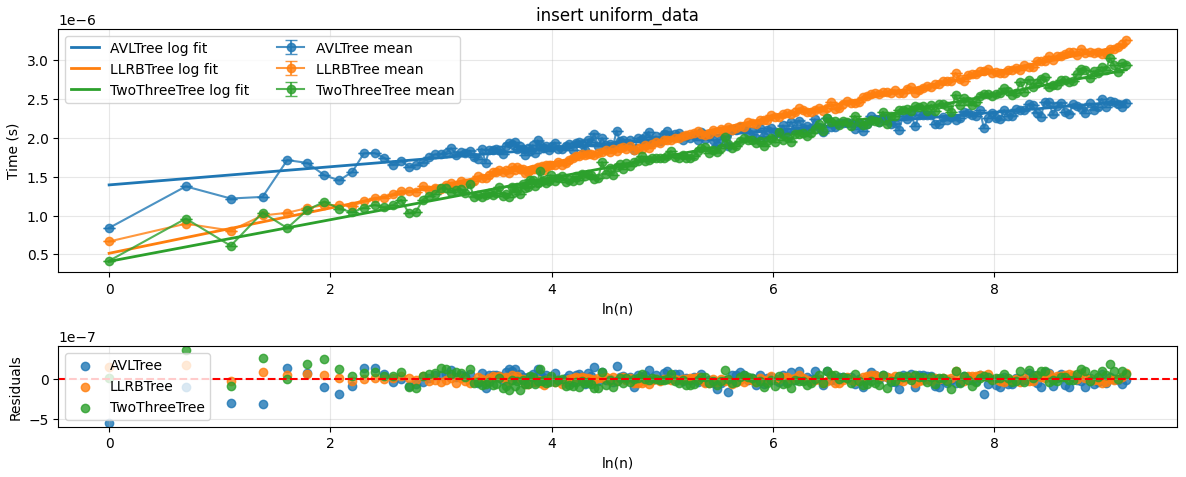
\includegraphics[width=\textwidth]{1.png}
        \vspace{-2em}
        \caption{Comparison of insertion time under uniformly distributed keys.}
        \label{fig:1}
    \end{minipage}
    \hfill
    \begin{minipage}{0.48\textwidth}
        \centering
        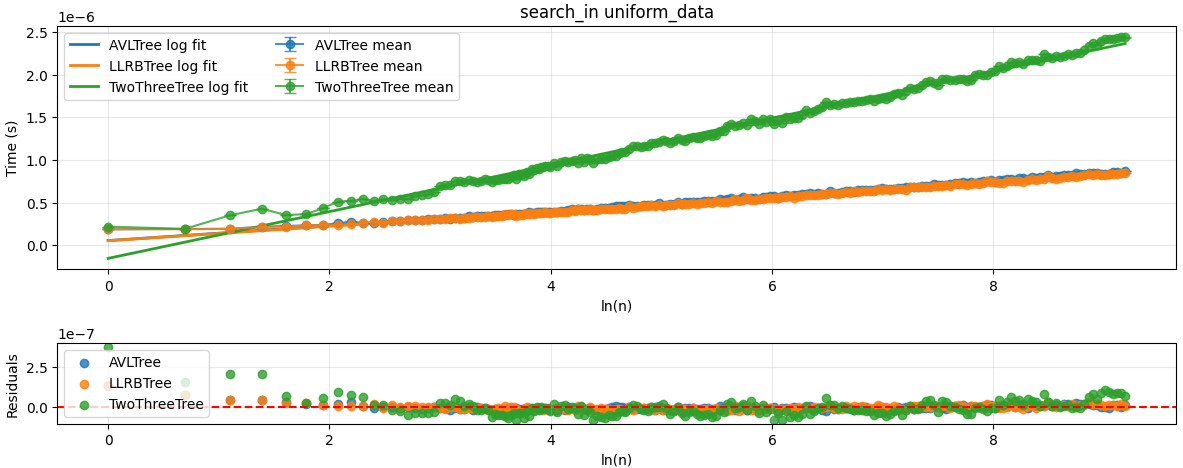
\includegraphics[width=\textwidth]{2.png}
        \vspace{-2em}
        \caption{Comparison of successful search time under uniformly distributed keys.}
        \label{fig:3}
    \end{minipage}
\end{figure}
\vspace{-2em}
\subsection{2-3 Tree}
With random input, the 2-3 tree gave low average insertion times - the gradient of the regression line for 2-3 insertions was approximately $2.22\times 10^{-7}$s - this can be interpreted as the extra time cost in increasing the number of nodes by a factor of $e$. Insertions trigger local split operations when a node becomes overfull which rarely propagate far up the tree, making them inexpensive.

The experiments showed that the main weakness of the 2-3 tree is search. For successful and unsuccessful searches, the fitted slopes had gradients ranging from $2.26\times 10^{-7}$s to $2.33\times 10^{-7}$s across all four key generation techniques - about three times larger than the corresponding AVL and LLRB slopes. The plots showed a step-like structure, especially for sorted and reverse-sorted data. Long horizontal segments correspond to periods where the tree height remains unchanged; steps appear when a new layer is created. The oscillating residuals suggest that even at the same height, performance strongly depends on the distribution of 2- and (more expensive to traverse) 3- nodes in the tree.
Ordered input revealed a second weakness: erratic insertion times. The scatter about the regression line was very high and the strength of the logarithmic fit deteriorated, with $R^2$ - a measure of how much variance the regression model captures - falling to about $50$ percent for sorted input and $43$ percent for reverse-sorted input. The spikes in the insertion graphs indicate the occurrence of cascading split operations through several layers of the tree. With sorted input, the cost of an insertion is determined by the number of 3-nodes above the rightmost leaf. If 2-nodes are viewed as binary 0s and 3-nodes as binary 1s, then sorted insertions behave like incrementing a binary counter, with binary carries causing split operations. So, expensive insertions occur at regular intervals, doubling in separation with every extra split. This explains the layered spike pattern observed in the sorted-input graph.
Overall, the 2-3 tree performs well when  average insertion throughput matters, but its search overhead and irregular insertion spikes make its runtime unpredictable, particularly when operating with worst-case data.

\begin{figure}[htbp]
    \centering
    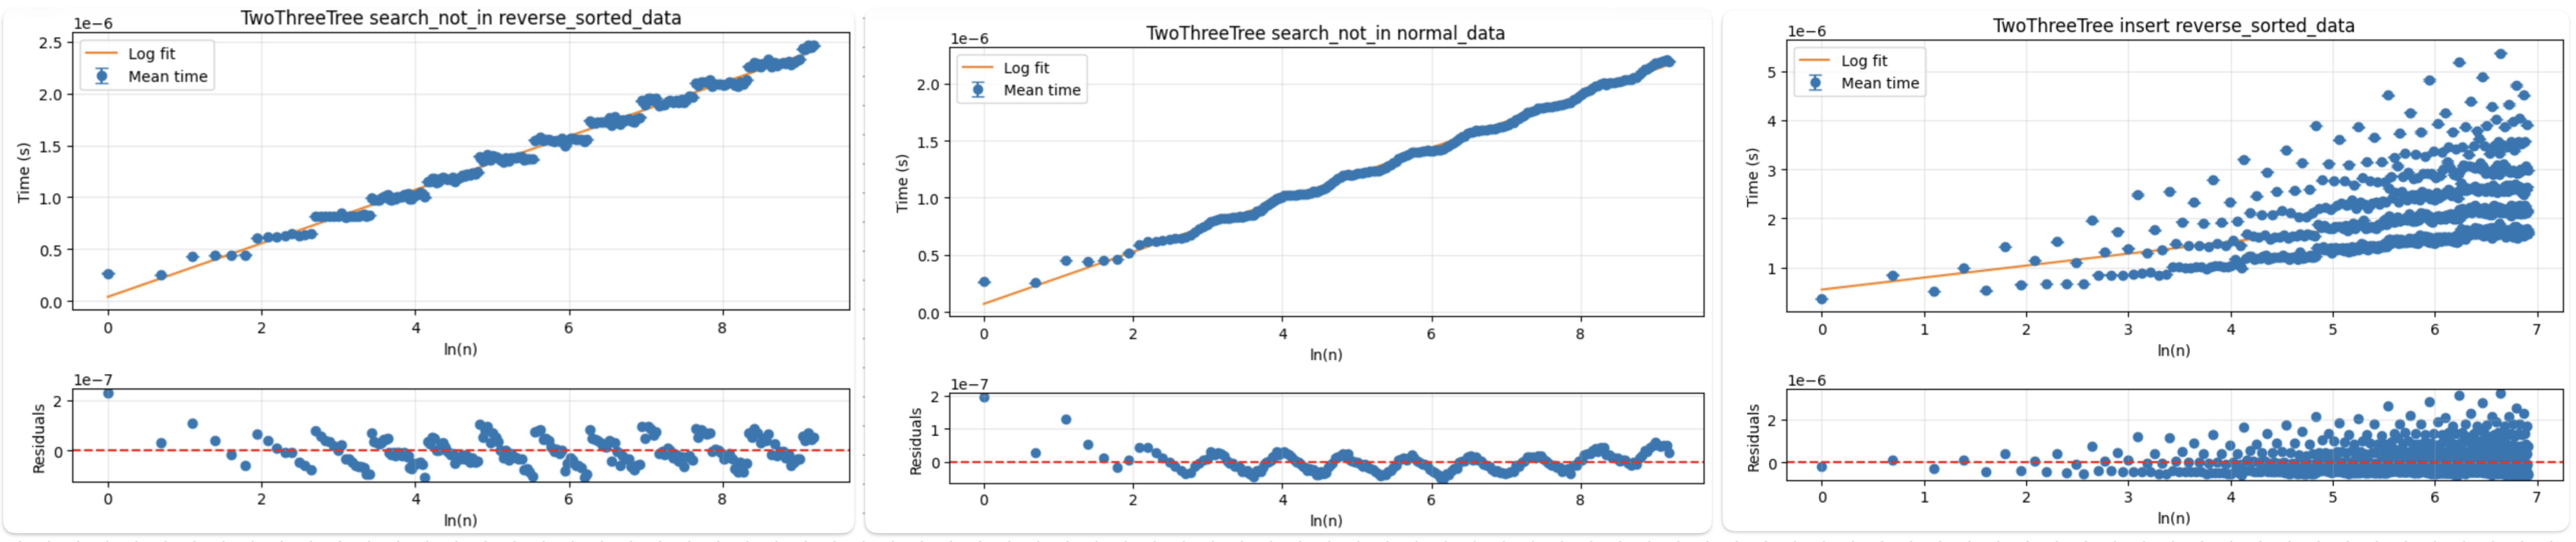
\includegraphics[width=0.6\textwidth]{4.png}
    \vspace{-1em}
    \caption{Representative 2-3 tree plots with residual patterns.}
\end{figure}

\vspace{-2em}
\subsection{LLRB Tree}
The LLRB tree performed strongly. For uniform and normal inputs, the insertion gradients are about $2.91 \times 10^{-7}$s. The search performance was also good. For successful searches, the fitted slopes are between $7.14 \times 10^{-8}$s and $8.06 \times 10^{-8}$s, and for unsuccessful searches between $6.30 \times 10^{-8}$s and $8.89 \times 10^{-8}$s.
This performance was consistent with expectations. The LLRB tree is a 2-3 tree isomorphism, using a BST representation, and cheap local rotations and colour flips to maintain balance. 

The black height invariant maintains a constant number of black nodes on any root-to-leaf path, and no two red nodes can be adjacent, meaning the LLRB guarantees any such path can have at most $2log_2n$ nodes. However, in practice, it seems the height was much closer to the optimum $log_2n$ case (see comparison with AVL trees in Section 3).

The limitation of the LLRB tree appears under reverse-ordered insertion. The graph's fitted slope rises to about $3.03 \times 10^{-7}$ and $R^2$ drops to about $0.75$, showing that although the trend remains logarithmic, the sequence of rotations and colour flips becomes more irregular when the inserted elements come with biased order.

Despite this, the LLRB was not hindered by inserting sorted data. The left-leaning invariant explains this asymmetry. Sorted keys are inserted as right children, which are immediately rotated to the left, without causing colour flips, whereas reverse-sorted keys are inserted as left children, and can cause cascading operations upwards.

Overall, the LLRB tree performs well, with fast searches and cheap insertions, but it is not robust when facing worst-case input.
\vspace{-1em}
\subsection{AVL Tree}
For AVL trees using random input, the fitted insertion gradients are about $1.17 \times 10^{-7}$s and $1.14 \times 10^{-7}$s, which are low. With sorted and reverse-sorted input, its insertion gradients stay low at $1.46 \times 10^{-7}$s and $1.27 \times 10^{-7}$s, and similar to the 2-3 trees, begin to show a layered spike pattern due to cascading rotations. Like the other structures, the AVL tree implementation uses early termination to avoid re-balancing further than it needs to.

Although the insertions are fast, the speed comes with a clear cost in predictability. The fit captures only about $91\%$ of the variance under random input, and only about $24\%$ under sorted and reverse-sorted input - explained by the fact that repeated insertions on one side of the tree cause several re-balancing operations to avoid lopsidedness and restore the AVL invariant. AVL trees maintain a symmetry at every node, and therefore perform best under input drawn from symmetrical distributions.

AVL insertions had the shallowest gradient of all three structures, but the highest intercept - $1.39 \times 10^{-6}$s (with uniform keys). This implies that the AVL balancing  imposes a fixed overhead on insertions, paid regardless of the tree's size, but the marginal cost of each extra layer of depth is the least. The strict balancing that ensures no node's sub-trees have heights differing by more than one is expensive to set up, but scales very well. There is an intersection between AVL's insertions and both 2-3's and LLRB's, covered in Section 3.

The cost of the AVL tree's strict balancing is justified by its speed in searching, where it is efficient and consistent. The successful search gradients range from about $8.55 \times 10^{-8}$ s to $9.81 \times 10^{-8}$s, while unsuccessful search slopes range from  $7.44 \times 10^{-8}$s to $8.60 \times 10^{-8}$s. These values are very close to those of LLRB - which has a similar implementation (though theoretically a different structure) - and the search fits are strong across all four key sampling techniques.
\begin{figure}[htbp]
    \centering
    \begin{minipage}{0.48\textwidth}
        \centering
        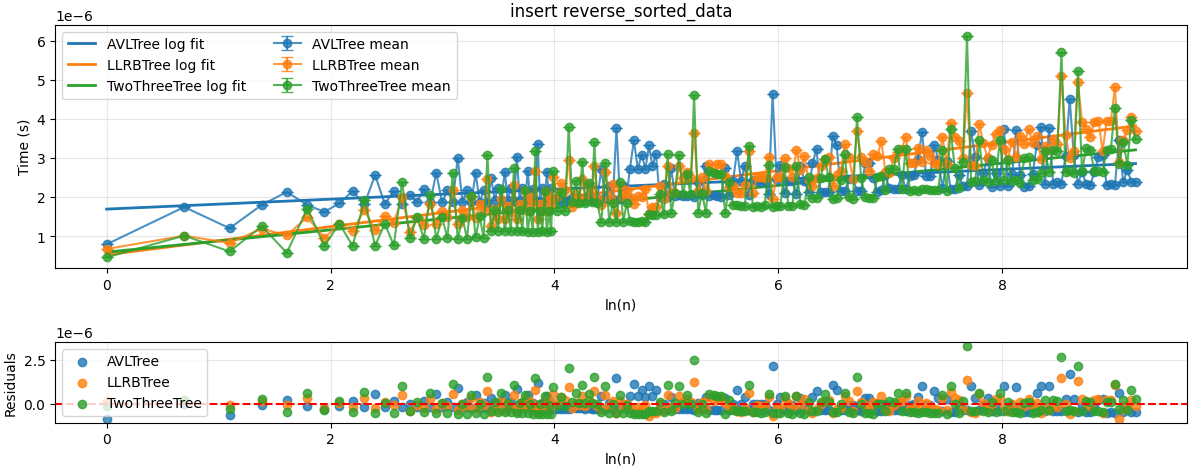
\includegraphics[width=\textwidth]{3.png}
        \vspace{-1em}
        \caption{Comparison of insertion time under reverse-sorted keys.}
        \label{fig:4}
    \end{minipage}
    \hfill
    \begin{minipage}{0.48\textwidth}
        \centering
        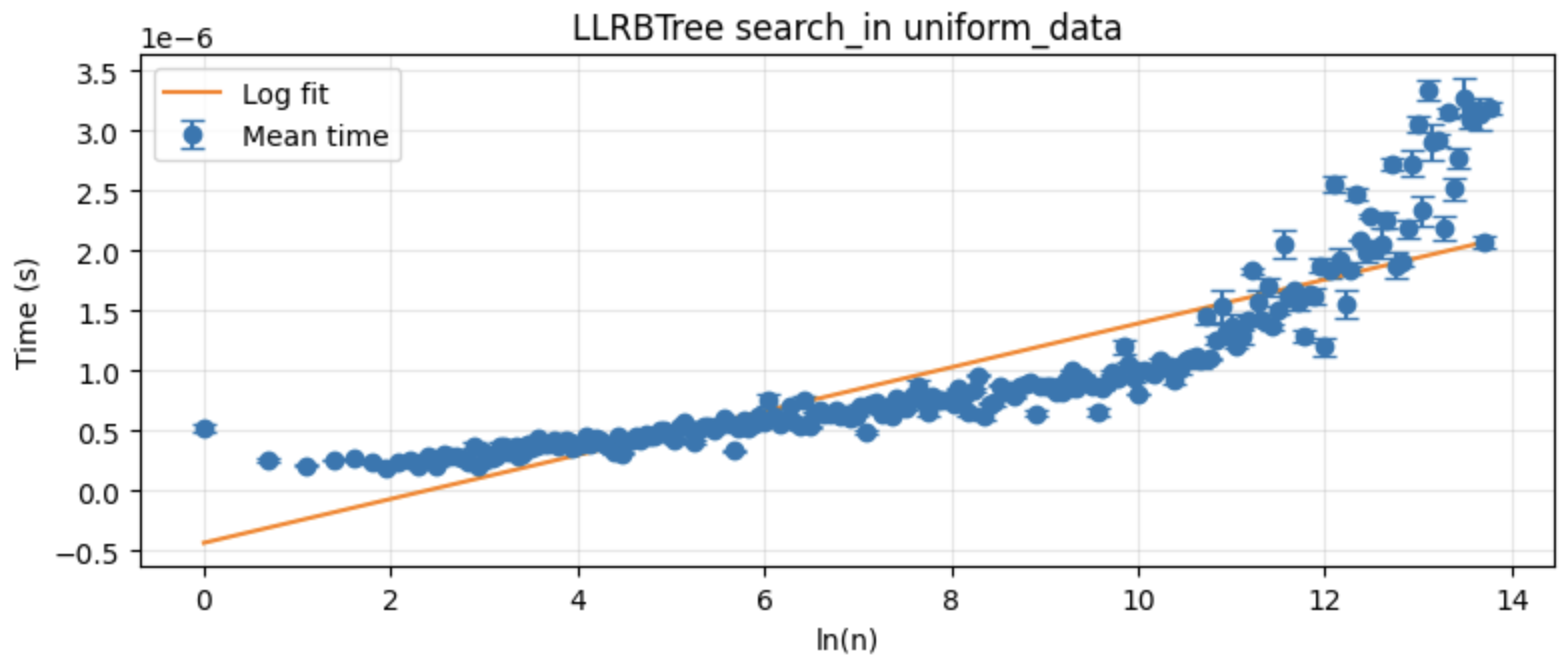
\includegraphics[width=\textwidth]{5.png}
        \vspace{-1em}
        \caption{Example of the observed upward bend in the graphs for large tree sizes.}
    \end{minipage}
\end{figure}
\vspace{-2em}
\section{Comparative assessment}
Each data structure showed strong logarithmic asymptotic growth. With random keys, the PMCC was greater than 0.99 for each plot, and the RMSEs were low (each < 5 nanoseconds) evidence of the fact that tree operations are indeed an $O(logn)$ operation in the average case.

The searching plots for AVL and LLRB trees showed nearly identical profiles - they are both binary trees with the same search algorithm which ignores colour and height, meaning comparisons at any node have the same cost, implying they have a similar depth on average.

LLRB trees have at most a depth of about $2log_2n$  \cite{sedgewick}, and AVL trees roughly $1.44log_2n$ \cite{mount}.
AVL trees maintain a costly invariant to achieve this lower upper-bound on depth but the results show that the theoretical bound on height fails to improve real-world searching performance. It is likely that drawing keys from even distributions had a self-balancing effect, giving both trees a better-than-expected balance, and explaining their similarities.

Despite still growing logarithmically, searching 2-3 trees was slower than AVL and LLRB, taking roughly $2.5$x the time in trees of size 10,000. This was a counter-intuitive result. 2-3 trees have a well-balanced structure. A search can take at most $2log_3N$ comparisons \cite{algorithms}, which is less than that of an AVL or LLRB tree. But these bounds are on the worst case: AVL and LLRB trees seemed to hold a better than worst case balance. And the 2-3 tree’s rigid structure means it always shows near-to-worst-case performance. Moreover, the 2-3 tree’s search uses Python list operations, which are notably slower than comparison-based operations used in the other trees. This could explain the performance gap.

Successful searches seemed to take the same amount of time as (or just less than) failed searches in every tree. In a balanced tree, most keys lie close to the leaves – half of the nodes in a balanced binary tree are leaf nodes, so this was not unexpected. 

For insertions with random inputs across all tree sizes, 2-3 trees just outperformed LLRB trees. The regression lines had very similar gradients, which means that the insertion costs scale similarly between the two implementations. But this similarity broke down with the sorted edge case, for which LLRB trees were actually faster than 2-3 trees. With reverse sorted input, the opposite was true - most likely a feature of the LLRB asymmetry.

Interestingly, AVL's insertion performance varied with the size of the tree. For small trees of size up to $e^5$ (roughly 100) nodes, AVL trees had the slowest implementation, but by $e^6$ (about 400) nodes, it was faster than the other two tree types. 

Across all trees, the data showed few outliers. $3.3$ per-cent of  insertions, and $4.0$ per-cent of searches were recorded as such in randomly constructed trees. Outliers were always positive ($> Q_3 + 1.5*IQR$). These spikes were random, and changed in distribution between runs of the program (even on the same trees). A supplementary test with disabled garbage collection dropped outlier rates substantially.

For large tree sizes, the plots showed a clear upwards bend. Figure 5 (page 4), shows a qualitative plot generated using $n$ = $10^6$, and a very low value of m = 3. It can be understood as the effect of cache misses. For trees of size roughly, $e^{10}$ (more than $10^5$ nodes), the storage occupied by the tree's nodes exceeds the L2 (see hardware specification) cache capacity, leading to poor cache locality and misses. As a result, error bars widen, and the gradient of the data points appear to sit on a new line, with an increased gradient. 

In memory, AVL nodes store an extra integer, and LLRB nodes have an extra boolean over a standard binary tree. The 2-3 tree node's overhead from using lists is expensive (about 2x as much in Python), although marginally counter-balanced by the ability of a 3-node to store two keys.

The results show different data structures are suited to different tasks. For insertion into small trees, 2-3 trees are the best. But they are quickly overtaken by AVL trees, which are better for trees with >500 nodes. AVL and LLRB trees are equally the fastest for searching. For search-heavy uses AVL and LLRB trees are the best choices. For insertions, if trees are kept small, 2-3 trees are a good option; if the trees are large, then AVL is better. Alternatively, if the scale of the tree is variable - or memory availability is tight-  LLRB offers a strong middle ground. All three implementations showed increased variance under adversarial input, but the average growth rates remained logarithmic.
\vspace{-2em}
\section{Team contributions}
\begin{tabular}{|l|l|l|l|}
\hline
Harry Mannix&  25005445&  2-3, section 3 and stats& ($33.33\%$)\\\hline
          Ben Dalton&            25012352&         AVL, section 1, testing&          ($33.33\%$)\\
%% more entries as needed
\hline
 Yuheng Zhu& 25105536& LLRB, section 2, graphs&($33.33\%$)\\\hline
\end{tabular}
\vspace{-1em}
\printbibliography
\end{document}
